\documentclass[journal]{IEEEtran}
\usepackage{amsmath,amssymb}
\usepackage{graphicx}
\usepackage{booktabs}
\usepackage{cite}
\usepackage{url}
\graphicspath{{../../Results/BlockTetris/}{../../Results/BlockTetris/circuit/}{../../Results/BlockTetris/sitra/}}

\begin{document}

\title{Block-Tetris: Electrically-Equivalent, Estimation-Aware Signal Control for Heterogeneous Urban Traffic Networks}

\author{Group~22, Department of Electrical and Electronics Engineering, Amrita Vishwa Vidyapeetham, Coimbatore, India% <- edit author list before submission
}

\maketitle

\begin{abstract}
We present Block-Tetris, a traffic-signal control algorithm built on an exact
charge-conservation equivalence between road traffic and an electrical network:
approach queues are capacitors, green phases are MOSFET taps, roads are delay lines
with a Zener-clamped storage limit, and network-level congestion management mirrors
power-system protection (attenuating relays, soft-start recovery, load shedding).
Traffic is quantised into 7.5\,m \emph{blocks} whose weights reflect the
heterogeneous Indian mix of two-, three- and four-wheelers and heavy vehicles.
Each junction places conflict-free sets of movements (``Tetris pieces'') to discharge
the most valuable stacked blocks; the network layer adds a per-road Kalman state
estimator fusing CCTV counts, CCTV queue views with a limited field of view, and
travel-time congestion flags, a three-level look-ahead transfer-capability
recursion that predicts spill-back, and reconstruction of a junction whose camera
has failed from its neighbours' messages.
We evaluate the algorithm on three independent test beds: a vehicle-level
simulator, a switched-circuit ``e-twin'' of a 16-junction grid with an N-1 fault
sweep, and an exact port of an existing published four-controller benchmark.
On that benchmark, with 30 paired seeds, Block-Tetris reduces average delay versus
the best existing controller (fully actuated) in 12 of 13 stochastic scenarios
($p<0.05$, Wilcoxon), by up to 25\,\% under platoons and sensor noise. On held-out
seeds and a held-out demand pattern on the grid it reduces delay by 46--81\,\%
versus fixed time and max-pressure in every run. We report the failures found
on the way and the fixes, including a gridlock mode of adaptive control under
oversaturation, and state the limitations that remain.
\end{abstract}

\begin{IEEEkeywords}
Adaptive traffic signal control, electrical equivalent, state estimation, Kalman filter,
heterogeneous traffic, spill-back, max-pressure, perimeter control, sensor failure.
\end{IEEEkeywords}

\section{Introduction}
Adaptive signal control in Indian cities faces three problems that the classical
systems SCOOT~\cite{hunt1982scoot} and SCATS~\cite{sims1980scats} were not designed
for: (i) highly heterogeneous traffic whose saturation flow depends on the share of
two-wheelers~\cite{indohcm2017}; (ii) shared approach lanes in which an overflowing
turn pocket blocks every movement behind it (head-of-line blocking); and (iii)
sensing limited to junction CCTV cameras that see only the first tens of metres of
each approach and occasionally fail. Network-wide, queue spill-back between closely
spaced junctions turns local congestion into gridlock.

Max-pressure control~\cite{varaiya2013maxpressure,kouvelas2014maxpressure} is
throughput-optimal under infinite storage, and capacity-aware variants normalise
pressure by link capacity to curb spill-back~\cite{gregoire2015capacity}. Perimeter
control based on the macroscopic fundamental
diagram~\cite{geroliminis2008yokohama,daganzo2008analytical} protects a region from
oversaturation by metering its boundary. State estimation on road networks has been
built on macroscopic flow models and Kalman filtering~\cite{wang2005ekf,kalman1960},
and travel times from probes have been used both for queue
estimation~\cite{ban2011queue} and as the input of max-pressure
control~\cite{mercader2020traveltime}.

This paper's contributions are:
\begin{enumerate}
\item An explicit electrical equivalent of a signalised network, built as a
switched-circuit solver whose every component has a traffic meaning
(Table~\ref{tab:equiv}), in which power-system tools (protection relays, N-1
contingency analysis, state estimation~\cite{abur2004se}, available transfer
capability) transfer directly.
\item The Block-Tetris controller: block-weighted queues, head-of-line-aware
attribution, exhaustive service with charge$\times$current phase selection, and a
network layer with predictive protection, Kalman estimation and neighbour-based
reconstruction of blind junctions.
\item A falsifiable evaluation on three independent test beds, including an exact
port of a previously published benchmark with four controllers, with held-out seeds,
a held-out demand pattern and paired significance tests; negative results are reported.
\end{enumerate}

\section{Electrical Equivalent of a Signalised Network}
\begin{table}[t]
\caption{Traffic--circuit equivalence used by the e-twin}
\label{tab:equiv}
\centering\small
\begin{tabular}{@{}ll@{}}
\toprule
Traffic & Circuit\\
\midrule
Stacked (queued) block weight $V$ & Capacitor voltage\\
Arrival flow & Current source\\
Green on a movement & MOSFET on (linear below $V_k$, saturation above)\\
Start-up lost time & Gate turn-on delay\\
Amber + all-red & Dead time (break-before-make)\\
Conflict matrix & Shoot-through interlock\\
Road (travel time $D$, storage $C$) & Delay line + Zener clamp at $C$\\
Shared lane before turn pockets & Series bottleneck (head-of-line)\\
Exit to outside & Current-limited load\\
Congestion alarm, per-hop attenuation & Protective relay, line impedance\\
Ramped recovery & Soft start / slew limiter\\
Boundary metering & Load shedding\\
\bottomrule
\end{tabular}
\end{table}
A road $l$ stores weight $z_l$ (moving plus stacked blocks). Charge conservation
(Kirchhoff's current law) gives
\begin{equation}
z_l(k+1)=z_l(k)+c^{\mathrm{in}}_l(k)-c^{\mathrm{out}}_l(k),
\label{eq:kcl}
\end{equation}
the same balance used by the cell transmission model~\cite{daganzo1994ctm}. A tap
(movement $m$) discharges $i_m=\min\{V_m,\; s_m\min(1,V_m/V_k)\,\Delta t,\;
C_e-z_e\}$, i.e.\ saturation current $s_m$, a linear region for nearly empty
stacks, and no current into a full exit road $e$ (Zener clamp). The solver integrates
the network at $\Delta t=1$\,s and is verified to conserve charge to machine
precision in every fault case.

\section{The Block-Tetris Algorithm}
\subsection{Blocks, weights and discharge time}
Each approach queue is quantised into 7.5\,m blocks. A block's weight is the sum of
its vehicles' weights (two-wheeler 0.2, three-wheeler 0.3, car 0.4, bus/truck 0.9);
only blocks that have \emph{landed} on the stack count as queue. The expected
discharge time of block $i$ is $t_i=W_i\tau_c$ with $\tau_c$ learned online per block
class from stop-line crossings, and a stack's clearing time is
\begin{equation}
T=L+\sum_i W_i\tau_{c(i)}+k\sqrt{\textstyle\sum_i\sigma_{c(i)}^2},
\end{equation}
the deviations combining in root-sum-square. Measured, $\tau\approx4.2$--$5.0$\,s per
weight unit per lane in our calibration, so the initial guess of 2\,s must be learned.
Samples taken while a queue ran dry or the exit was blocked are discarded.

\subsection{Tetris placement at a junction}
The 16 movements of a four-arm junction (left, straight, right, U-turn per arm; left-hand
traffic) are drawn as chords; two conflict if their chords cross or merge. This yields
53 maximal conflict-free sets. Vehicles stuck in a shared section are attributed to
the pocket that blocks them. The selected set is served \emph{exhaustively}: until its
stacks fall below a low mark with no platoon arriving, its taps pass no current
(blocked exit or lamp fault), or $g_{\max}$; the next set maximises
$\sum_m (V_m + a\,V_m\,\mathrm{age}_m)\,\hat s_m\,(1-p_{e(m)})$, i.e.\ stored charge
times learned discharge current, with an age term against starvation and the
downstream pressure $p$. Minimum green is raised to 35\,s when the junction is
saturated. Exhaustive service relates the controller to polling
systems~\cite{takagi1986polling}.

\subsection{Network layer}
\emph{Protection.} Road loading $z_l/C_l$ above 0.8 latches an alarm (released at 0.6,
Schmitt trigger) whose pressure propagates upstream attenuated by 0.5 per hop and
recovers with a ramp; phase scores are multiplied by $(1-p)(1-(z/C)^2)$, a smooth
back-pressure in the spirit of capacity-aware control~\cite{gregoire2015capacity}.
Boundary inflow is metered when interior accumulation exceeds 0.30 of storage,
following perimeter control~\cite{geroliminis2008yokohama}; above 0.45 every junction
rotates through all arms (emergency mode), and roads whose pressure exceeds 0.9 trigger
diversion of the traffic that intended to enter them.

\emph{State estimation.} Each road has a scalar Kalman filter~\cite{kalman1960} with
(\ref{eq:kcl}) as process model, CCTV counts as inputs, process noise
$Q=\epsilon^2(c^{\mathrm{in}}+c^{\mathrm{out}})+q_0$, and measurements from the CCTV
view: if the stack $q$ fits in the field of view $W$, $y=q+\hat\lambda D$ (stack plus
estimated moving blocks); if it overflows, the inequality $z\ge W+\tfrac12\hat\lambda D$.
Readings with normalised innovation $\nu^2/S>9$ are rejected as bad data, as in
power-system state estimation~\cite{abur2004se}.

\emph{Look-ahead transfer capability.} With learned service current $\mu$, predicted
flows $f_{u,k}$ from road $u$ to exit $e_k$ and $F_e=\sum f$, the acceptance rate and
discharge capability are computed $D=3$ levels downstream over horizon $H=120$\,s:
\begin{align}
A_e^{(0)}&=\mu_e+\max(0,0.9C_e-z_e)/H,\\
C_u^{(d)}&=\min\Big(\mu_u,\ \min_k \tfrac{f_{u,k}}{F_{e_k}}\,A_{e_k}^{(d-1)}/r_k\Big),\\
A_u^{(d)}&=C_u^{(d)}+\max(0,0.9C_u-z_u)/H,
\end{align}
the inner minimum expressing head-of-line coupling through the turn ratios $r_k$. The
predicted load $(z+H(F-C^{(D)}))/C$ replaces the present load in the protection layer,
so restrictions two or three roads downstream slow the inflow before the queue arrives.

\emph{Blind junctions.} When a junction's camera fails its stacks are rebuilt from
neighbour messages: inflow equals upstream send counts delayed by the travel time,
outflow is predicted from its own signal state and learned $\tau$, and downstream
landing counts $D$ seconds later correct the prediction. The junction keeps running
Block-Tetris on the rebuilt stacks and falls back to a fixed rotation only while the
network accumulation exceeds 0.40.

\section{Experimental Setup}
\emph{Test bed A (vehicle level):} a five-junction chowrasta, 16 movements per junction,
turn pockets, stochastic headways, eight congestion scenarios, eight seeds.
\emph{Test bed B (e-twin):} the circuit solver on a $4\times4$ grid (16 junctions,
80 roads), N-1 sweep of 88 single faults (every road closed, every exit cut to 5\,\%,
every gate surged $\times2.2$, slowed approaches) at 1.9$\times$, 2.3$\times$ and
2.9$\times$ the normal demand. \emph{Test bed C (published benchmark):} an exact Python
port of an existing four-controller benchmark (SITRA-MPC, Webster, fully actuated,
max-pressure; scenarios T1--T14) that reproduces its published average delays to
0.002\,\%. Statistics use paired seeds, the Wilcoxon signed-rank test and bootstrap
95\,\% intervals; held-out validation uses seeds 11--20 and a demand pattern not used in
tuning (north--south $\times1.4$, east--west $\times0.7$, Gaussian peak).

\section{Results}
\subsection{Published benchmark (test bed C)}
\begin{table}[t]
\caption{Average delay (s/veh), 30 paired seeds, Block-Tetris vs fully actuated (best existing)}
\label{tab:sitra}
\centering\small
\begin{tabular}{@{}lrrrrr@{}}
\toprule
Scenario & Actuated & Block-Tetris & $\Delta$ & 95\,\% CI & $p$\\
\midrule
T1 low & 12.1 & 11.8 & $-0.3$ & $[-0.6,0.0]$ & 0.05\\
T2 moderate & 18.5 & 17.4 & $-1.1$ & $[-1.6,-0.6]$ & $4\!\times\!10^{-4}$\\
T3 high & 41.4 & 37.3 & $-4.1$ & $[-4.8,-3.5]$ & $<10^{-8}$\\
T4 oversaturated & 122.7 & 112.8 & $-9.9$ & $[-11.6,-8.3]$ & $<10^{-8}$\\
T5 step & 28.9 & 26.2 & $-2.7$ & $[-3.3,-2.1]$ & $<10^{-8}$\\
T7 surge & 21.3 & 17.5 & $-3.9$ & $[-4.4,-3.4]$ & $<10^{-8}$\\
T8 congested start & 50.6 & 49.1 & $-1.5$ & $[-2.1,-1.0]$ & $2\!\times\!10^{-6}$\\
T9 incident & 20.2 & 19.1 & $-1.2$ & $[-1.6,-0.8]$ & $10^{-5}$\\
T10 blockage & 22.5 & 21.2 & $-1.3$ & $[-2.0,-0.6]$ & $10^{-3}$\\
T11 platoon & 40.3 & 32.7 & $-7.6$ & $[-8.7,-6.6]$ & $<10^{-8}$\\
T12 sensor stuck & 22.0 & 24.7 & $+2.7$ & $[-0.5,6.1]$ & 0.35\\
T13 sensor noise & 27.7 & 20.6 & $-7.0$ & $[-7.8,-6.2]$ & $<10^{-8}$\\
T14 lamp fault & 21.9 & 19.2 & $-2.7$ & $[-3.8,-1.7]$ & $5\!\times\!10^{-6}$\\
\bottomrule
\end{tabular}
\end{table}
Table~\ref{tab:sitra}: Block-Tetris is significantly better in 12 of 13 stochastic
scenarios; the stuck-sensor case T12 is not significant. Against SITRA-MPC, Webster and
max-pressure the reductions are larger (Fig.~\ref{fig:sitra}).
\begin{figure}[t]\centering
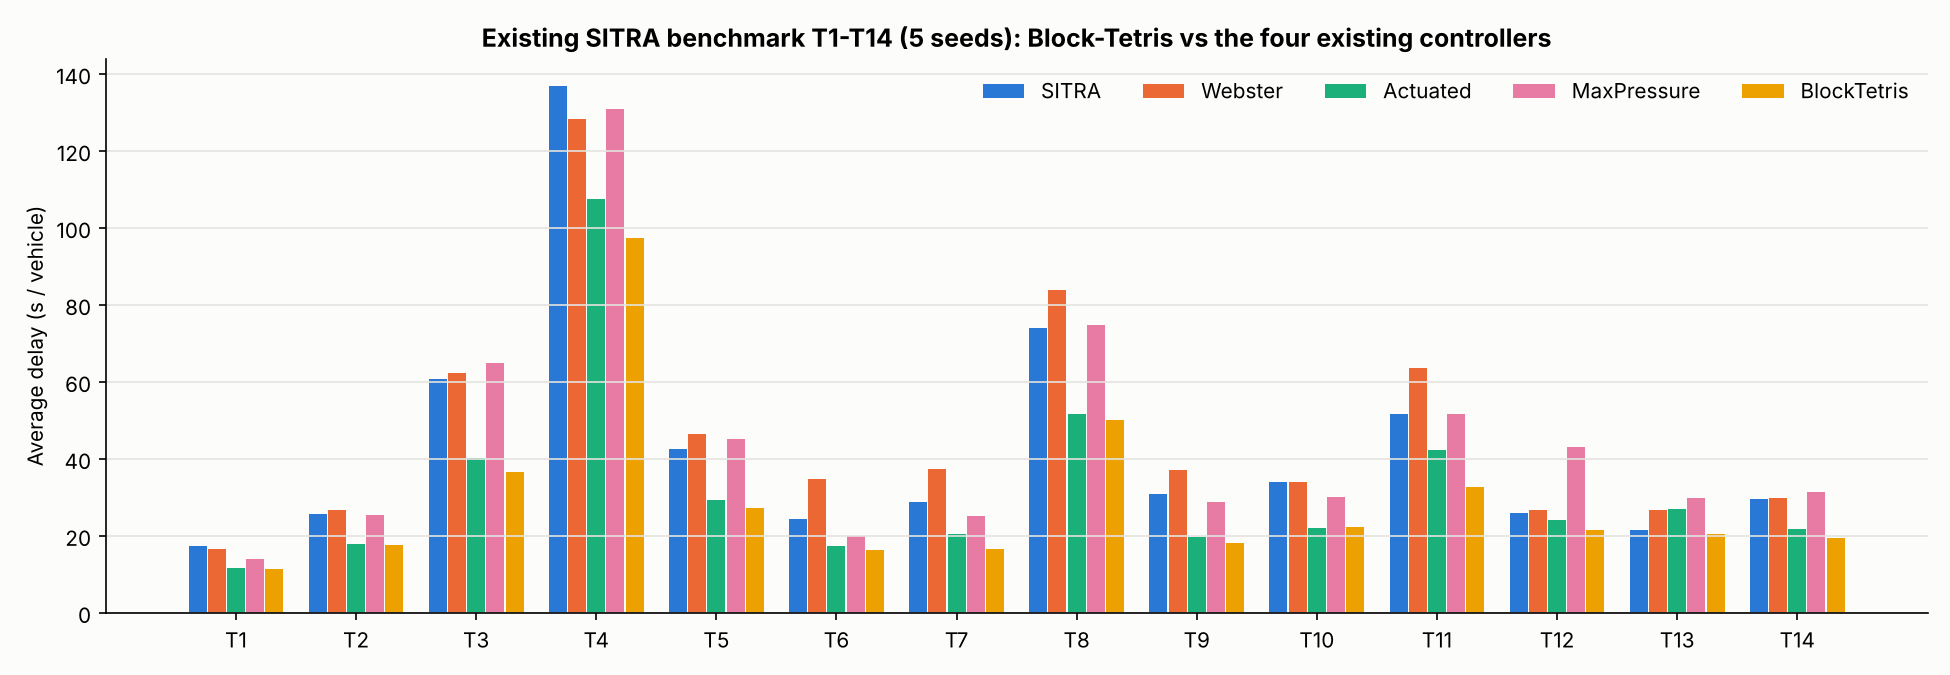
\includegraphics[width=\columnwidth]{fig9_sitra_benchmark.png}
\caption{Published benchmark T1--T14, five seeds: Block-Tetris vs the four existing controllers.}
\label{fig:sitra}\end{figure}

\subsection{Network e-twin (test bed B)}
On held-out seeds and the held-out demand pattern (1.9$\times$ demand), mean delay is
Fixed 474\,s, max-pressure 577\,s, Block-Tetris v3 252\,s, v4 255\,s, and v6 with
realistic 60\,m CCTV 291\,s; with a road closed 1420, 1070, 283, 268 and 310\,s; every
Block-Tetris variant beats both baselines in 10/10 runs ($p=0.002$).
Fig.~\ref{fig:cap} shows that v3 is the only controller whose throughput never falls
below fixed time up to 4$\times$ demand.
\begin{figure}[t]\centering
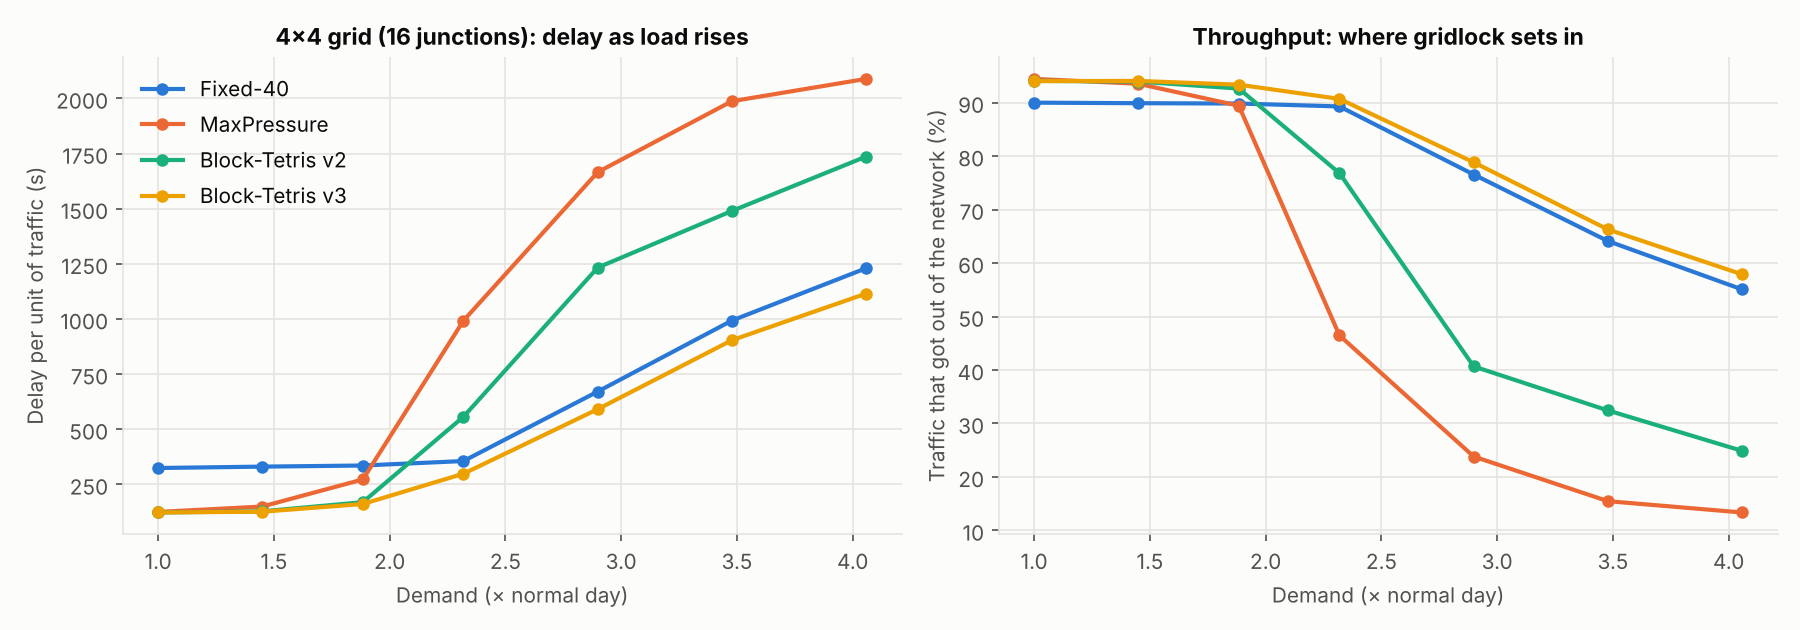
\includegraphics[width=\columnwidth]{fig7_capacity_curve.png}
\caption{4$\times$4 e-twin: delay and throughput vs demand.}
\label{fig:cap}\end{figure}

\emph{Look-ahead (v4 vs v3).} The predictive layer helps specifically with road closures under
overload: $-33\,\%$ at 2.9$\times$ ($p=0.006$, 9/10) and $-22\,\%$ at 2.3$\times$ (not
significant); on fault-free days the difference is not significant. Measured passively,
the predictor warns of 88--96\,\% of spill-backs 66--131\,s in advance with 7--15\,\%
precision.

\emph{Realistic sensing (v6).} Limiting CCTV to a 60\,m view raises v5's delay by
42\,\% at 2.3$\times$ (344$\to$489\,s); the v6 estimator recovers it to 376\,s, and on
held-out seeds v6 beats v5-with-CCTV by 11--14\,\% (10/10, $p=0.002$). With up to four
central cameras dead, neighbour reconstruction cuts the blind junctions' queue error by
65--75\,\% versus holding the last frame and gives the lowest delay in five of six
cases.

\subsection{Failures found and fixed}
The algorithm as first specified gridlocked even under normal demand (test bed A); an
ablation attributes most of the repair to rolling re-placement and head-of-line
attribution. Under oversaturation adaptive control thrashed (15\,s greens, 37\,\% lost
time) and filled interior roads into gridlock loops; this was fixed by current-based
switching, saturation green, back-pressure, metering and emergency rotation. Applying
the look-ahead throttle directly to phase scores, and converting lagged travel times to
queue lengths by Little's law~\cite{little1961}, both made control worse and were
rejected.

\section{Discussion and Limitations}
\emph{Stability.} Unlike max-pressure~\cite{varaiya2013maxpressure} Block-Tetris has no
proof of maximal stability; its guarantees are empirical. Phases are not served in a fixed
cycle, which drivers may find less predictable~\cite{levin2020cyclical}; the age term and
emergency rotation bound waiting but a cyclical variant is future work.
\emph{Travel-time data.} Aggregated, lagged travel times correlated only 0.3 with
per-road stacks under signal cycling, consistent with per-cycle probe methods requiring
finer data~\cite{ban2011queue,mercader2020traveltime}; we use them only as a congestion flag.
\emph{Model fidelity.} The e-twin is a fluid model; pedestrians, lane indiscipline and
re-routing beyond diversion orders are not modelled; capacities and weights are assumed and
must be calibrated with field counts~\cite{indohcm2017}. Thresholds were tuned on the
evaluation networks; held-out tests mitigate but do not remove this risk.

\section{Conclusion}
Treating a signalised network as an electrical network gives a compact, physically
interpretable controller and a set of proven power-system tools for protection, estimation
and contingency analysis. Block-Tetris outperforms the best controller of an existing
benchmark with statistical significance and is robust to road closures, oversaturation,
limited CCTV and camera failures in simulation. Field calibration with Coimbatore counts and
a shadow-mode pilot are the next steps.

\section*{Code and Data Availability}
All simulators, controllers, experiment scripts and raw results are in the
project repository (\texttt{blocktetris/}, \texttt{Results/BlockTetris/});
every table is regenerated by the corresponding script
(\texttt{sitra\_bench}, \texttt{validation}, \texttt{validation\_overload},
\texttt{cctv\_experiments}, \texttt{blind\_experiments}). Each earlier
algorithm version remains executable for comparison.

\bibliographystyle{IEEEtran}
\bibliography{refs}
\end{document}
